{
After producing the suitable set of features for each of the 
physical parameters we are interested in, the next step will be
to produce the effective model becoming useful to predict those 
parameters. 
The researcher will decide how many features will be used in the 
multivarite model proposed to explain the physical parameter for 
the learning dataset (BT\_Settl). 
The models produced by this way will be used to forecast the 
physical parameters for the IRTF library.

As a matter of analysis different cross-comparison tests
were performed, like performance against the parameters
infered from the closer BT\_Settl by using the $\chi^2$ distance 
with different SNR. Comparisons were indeed performed against 
other inductive Machine Learning strategies, like project 
the spectra in a smaller feature dimensional space by using
Independent Component Analysis (ICA) and then, developping 
a regression model based on such features (see \ref{ssub:GM_BPG}).
For the special case of temperature a comparison between the
temperature and the known spectral subclase makes possible to 
analyze the quality of the forecasted estimations (see \ref{ssub:TLSB}).
}

\subsection{Models considered.}
\label {ssub:models}
{
For the models to be built, the same strategy was used for all the 
three physical parameters $(T_{eff}, log(g), met)$ 
and it was to use non linear methods for modellization.
As a classical regression problem several linear and non-linear
modelling techniques with specific research for 
adequate parameters per method when required, were considered:
\begin{itemize}
 \item {Generalized Additive Models \emph{(GAM)}.}
 \item {Bagging with Multiadaptative Spline Regression Models \emph{(MARS)}.}
 \item {Random Forest Regression Models \emph{(RF)}.} 
 \item {Gradient Boosting with Regression Trees \emph{(BOOSTING)}.}
 \item {Generalized Boosted Regression Models \emph{(GBM)}.}
 \item {Support Vector Machine Models with Gaussian Kernel \emph{(SVM)}.}
 \item {MLP Nerural Networks \emph{(NNET)}.}
\end{itemize}

}

{
Comparison of performance between sets of features for temperature 
derived from the GA based strategy can be analyzed, 
over the same testing dataset of BT\_Settl and it was depicted 
in Table~\ref{tab:model_TSD}.

\begin{table}
\begin{center}
\begin{tabular}{rrrrrrr}
  \hline
  SNR & Features & SVM & RF & GAM  & MARS  \\
  \hline
  \multirow{2}{*}{50}  &  Cesetti et al. & 81.6 &  83.3 & 163.5 & 91.9 \\
      &  GA             & 91.4 & 82.2 & 161.1  & 91.9  \\
  \multirow{2}{*}{10}  &  Cesetti et al. & 135.8 & 138.5 & 268.8 & 166.8  \\
      &  GA             & 123.2 & 122.6 & 212.6 & 130.9  \\
   \hline
\end{tabular}
\caption { RSME for different models predicting $T_{eff}$ [K].} 
\label{tab:model_TSD} 
\end{center}
\end{table}

After calculating the bartlett test for both cases of SNR it was 
seen that variances are homogeneous since p > 0.05, and 
the Flinger-Killen shows that homkedascity is verified, 
then F-ANOVA test makes clear that there is no significative 
difference between models. Then, it is possible to conclude
that quality of features from both sources are equivalent
regarding modeling capability, even when GA only has proposed five
features and Cesetti et al. requires seven features.

}

\subsection{Full Spectra Oriented Models}
\label {ssub:GM_BPG}
{
As an alternative to build modles based on bandpasses, 
a similiar methodology to the one depicted in (\cite{2013A&A...550A.120S})
was implemented.

For the projection an Independend Component Analysis (ICA) with ten dimensions
was used and for Temperature regression an optimized SVM 
with parameters of C=10 and $\epsilon$=0.001.

Considering the Gravity case, the most suitable ICA had twentysix dimensions and the 
best SVM parameters were C=1000 and $\epsilon = 0.001 $. This was the same case
for Metallicity.

In terms of interpretation, this methodology looks to predict the physical paramenters
by considering the whole star spectrum instead of information provided 
by specific bands. Thus it can be interesting to analyze suitability 
for prediction against the other approach.

In the same sense it was decided to consider direct selection, which is
also a technique based on the whole espectrum but, instead of regressing
specific parameters, the closest labeled spectrum to the one 
under analysis is identified by a $\chi^2$ distance.
This becomes possible as interpolation between labeled spectra can be
easily performed.

}

\subsection{Temperature model based on Spectral Subtype.}
\label {ssub:TLSB}
{
% Luis ¿esto lo explicas tu?
}

\subsection{Temperature Model for $T_{eff}$.}
\label {ssub:teff_model}
{
After training the set of models by using labelled BT\_Settl dataset, those models 
were used to predict the IRTF temperature.
The authors were interested in understand how relevant the SNR factor 
becomes in terms of model training and in terms of forecasting. Thus, 
performance analysis between direct spectra comparison by means of $ \chi^2 $ and 
models using bandpass features was carried out.
Only the most five relevant features based of the exhibited fitness were considered.
Comparisons between models trained with different SNR and tested against 
features from other SNR were performed. Notation FTab will mean Forecasted temperature
when a accounts for the SNR of the feature set considered for the forecast and b
accounts for the SNR used for training the model. Both a and b have the 
meaning of 0 for SNR of $\infty$, 1 for SNR=10 and 5 for SNR=50.
Training was performed by 10 fold cross valdiation technique, making possible 
to select de convenient model.

Forecast quality of models was tested by the error against the temperature 
estimated based on the Spectral Subtype for each of 
the IRTF available spectra (see \ref{ssub:TLSB}).
Both Root Mean Squared Error (RMSE) and Mean Absolute Error (MAE) where calculated 
and it is presented in the table~\ref{tab:model_Tvar}.

\begin{table}[ht]
\centering
\begin{tabular}{rrr}
  \hline
 & RMSE & MAE \\ 
  \hline
chi2d\_10 & 428.83 & 261.53 \\ 
  chi2d\_50 & 426.31 & 267.77 \\ 
  FT00 & 427.33 & 307.38 \\ 
  FT01 & 366.82 & 248.38 \\ 
  FT05 & 429.02 & 299.58 \\ 
  FT10 & 438.61 & 327.93 \\ 
  \textbf{FT11} & \textbf{410.11} & \textbf{291.79} \\ 
  FT15 & 427.34 & 316.98 \\ 
  FT50 & 420.70 & 300.69 \\ 
  FT51 & 375.82 & 259.02 \\ 
  FT55 & 430.10 & 303.54 \\ 
   \hline
\end{tabular}
\caption { RSME \& MAE for different Random Forest models predicting $T_{eff}$ [K].} 
\label{tab:model_Tvar} 
\end{table}

From this comparison several things arise:
\begin{itemize}
 \item {The behavior of $\chi^2$ distance is quite stable against SNR 
	in the original dataset (BT\_Settl) with a slightly better global 
	performace in fovour of SNR=50.}
 \item {Models trained with different SNR=$\infty$ have similar performance but heavy 
	differences appear when SNR features are considered.}
 \item {When synchronous behavior is observed FT00, FT11, FT55, the better SNR is 10.}
 \item {Best set of features to be used for forecast are those from SNR=$\infty$ (FT0b).}
 \item {As a conclusion the better performance was produced by FT01, followed by the FT51.}
\end{itemize}

However a comparison between performance of different type of models with the same
set of features has been performed. In table~\ref{tab:models_T_rmse} the RMSE is presented for 
those different models and in table~\ref{tab:models_T_mae} the MAE is presented.

\begin{table}[ht]
\centering
\begin{tabular}{rrrrrrrr}
  \hline
 & rf & gbm & boosting & svm & gam & nnet & mars \\ 
  \hline
  FT00 & 427.33 & 431.65 & 419.67 & 376.60 & 1116.91 & 751.23 & 552.21 \\ 
  FT01 & 366.82 & 364.80 & 356.12 & 302.88 & 385.65 & 371.68 & 444.40 \\ 
  FT05 & 429.02 & 430.20 & 420.40 & 393.73 & 433.09 & 2514.35 & 492.70 \\ 
  FT10 & 438.61 & 443.49 & 446.94 & 321.55 & 2201.21 & 1269.82 & 590.28 \\ 
  FT11 & 410.11 & 407.80 & 400.37 & 359.50 & 430.10 & 419.32 & 487.69 \\ 
  FT15 & 427.34 & 439.24 & 428.89 & 317.02 & 371.22 & 2738.34 & 509.44 \\ 
  FT50 & 420.70 & 427.82 & 420.78 & 326.10 & 3742.74 & 1243.80 & 551.57 \\ 
  FT51 & 375.82 & 370.44 & 388.54 & 312.66 & 390.91 & 437.61 & 448.20 \\ 
  FT55 & 430.10 & 431.68 & 424.52 & 361.94 & 378.87 & 432.15 & 490.68 \\ 
  chi2d\_10 & 428.83 & 428.83 & 428.83 & 428.83 & 428.83 & 428.83 & 428.83 \\ 
  chi2d\_50 & 426.31 & 426.31 & 426.31 & 426.31 & 426.31 & 426.31 & 426.31 \\ 
   \hline
\end{tabular}
\caption { RSME for different models predicting $T_{eff}$ [K].} 
\label{tab:models_T_rmse} 
\end{table}

\begin{table}[ht]
\centering
\begin{tabular}{rrrrrrrr}
  \hline
 & rf & gbm & boosting & svm & gam & nnet & mars \\ 
  \hline
YTn00 & 307.38 & 311.42 & 303.22 & 282.06 & 836.62 & 531.86 & 349.10 \\ 
  FT01 & 248.38 & 250.10 & 246.03 & 221.95 & 258.83 & 255.74 & 267.70 \\ 
  FT05 & 299.58 & 305.64 & 301.72 & 285.80 & 314.94 & 2378.76 & 335.36 \\ 
  FT10 & 327.93 & 331.29 & 334.81 & 254.95 & 1514.75 & 1192.57 & 389.98 \\ 
  FT11 & 291.79 & 291.86 & 291.25 & 272.35 & 305.62 & 304.18 & 319.47 \\ 
  FT15 & 316.98 & 327.49 & 314.83 & 250.50 & 271.28 & 2636.53 & 353.85 \\ 
  FT50 & 300.69 & 307.18 & 308.42 & 252.72 & 2559.17 & 1049.08 & 361.82 \\ 
  FT51 & 259.02 & 255.30 & 272.60 & 226.32 & 263.27 & 318.01 & 274.19 \\ 
  FT55 & 303.54 & 309.75 & 307.33 & 269.07 & 274.98 & 308.48 & 333.29 \\ 
  chi2d\_10 & 261.53 & 261.53 & 261.53 & 261.53 & 261.53 & 261.53 & 261.53 \\ 
  chi2d\_50 & 267.77 & 267.77 & 267.77 & 267.77 & 267.77 & 267.77 & 267.77 \\ 
   \hline
\end{tabular}
\caption { MAE for different models predicting $T_{eff}$ [K].} 
\label{tab:models_T_mae} 
\end{table}


In Figure~\ref{fig:comp01} the relationship between Temperature estimated from 
the GA model proposed features with SNR=50 and features from SNR=$\infty$ 
and the Temperature estimation from spectral subtype 
in comparison with the $chi^2$ with SNR=50 can be seen.

\begin {figure}
 \centering
 \begin{subfigure}{.85\textwidth}
  \centering
  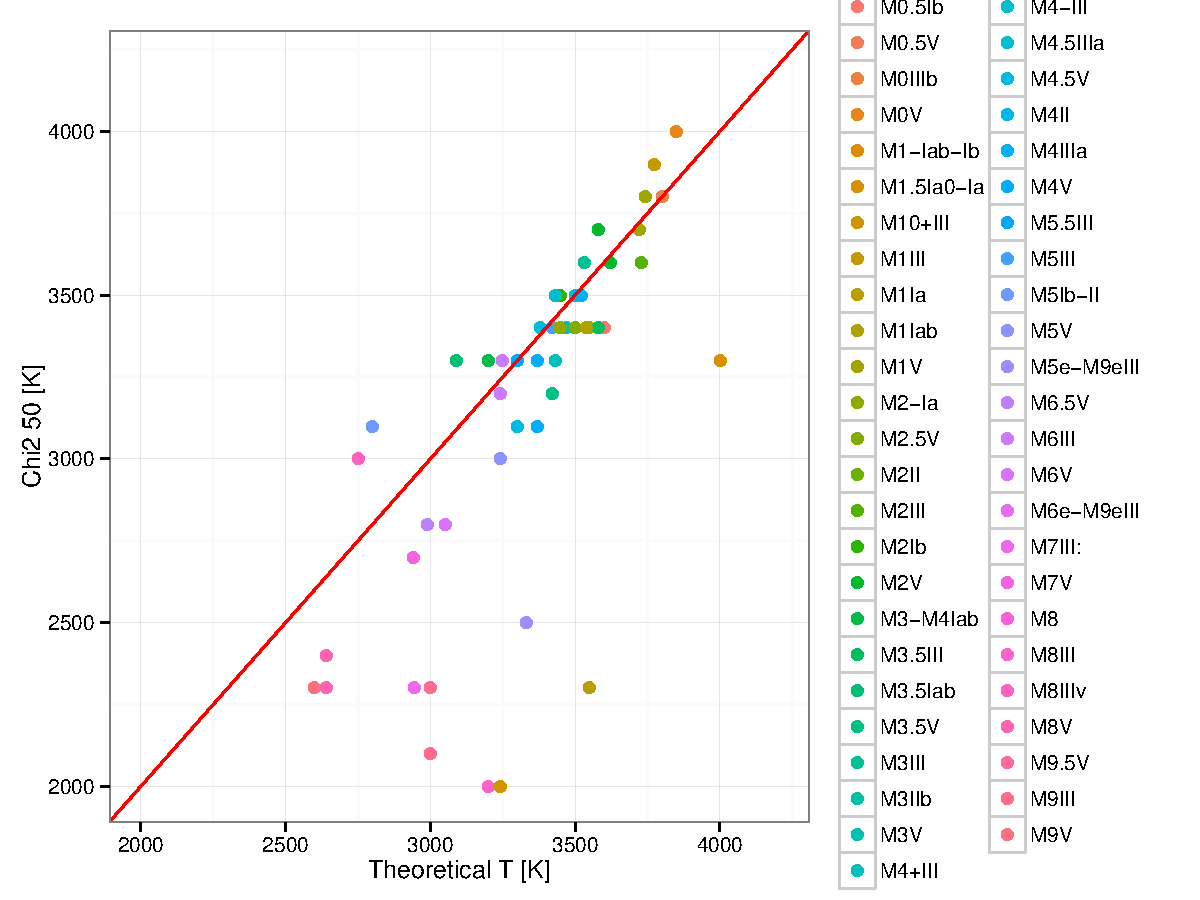
\includegraphics[width=13cm]{figs/T_chi50_Tst.pdf}
  \caption{Comparison between Temperature estimations from Spectral Subtype 
 in x axis and the closest BT\_Settl spectra by $\chi^2$ at SNR=$50$ on y-axis}
 \label{fig:chi2_50_spt}
 \end{subfigure}
  \begin{subfigure}{.85\textwidth}
  \centering
  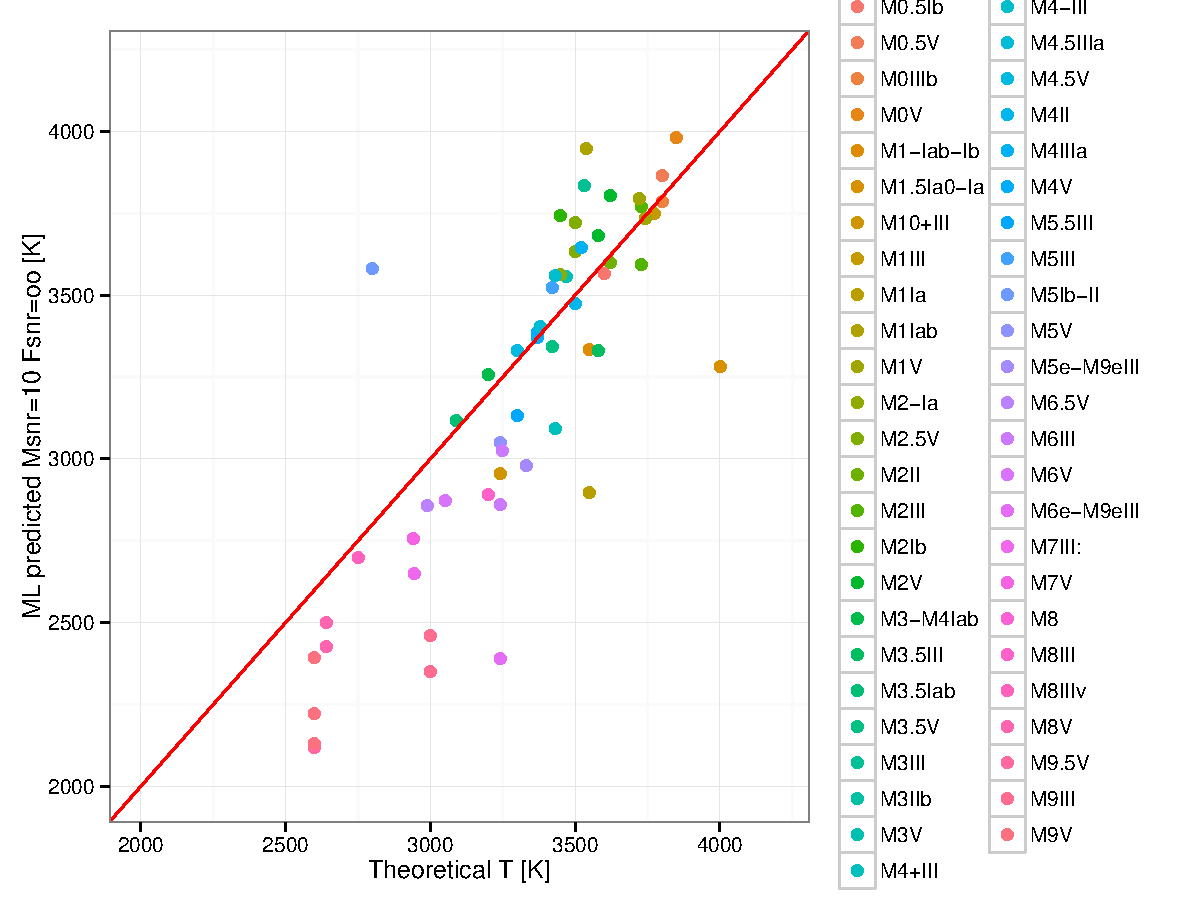
\includegraphics[width=13cm]{figs/T_svm_10_TsP.pdf}
  \caption{Comparison between Temperature estimations from Spectral Subtype 
 in x axis and the Support Vector Machines for Ga based features trained with BT\_Settl 
 at SNR=$\infty$ and features for forecasting at SNR=10 on y-axis}
 \label{fig:ga_too50ga_spt}
 \end{subfigure}
 \label {fig:comp01}
 \caption{Performance comparison between the $chi^2$ based selection 
          and the band oriented features}
\end {figure}
%
% No le añado más discusión porque habría que interpretar algunas estrellas.
%

% En kile ^D Comenta y ^MayD descomenta
%
% Similarly Figure~\ref{fig:t10ga_tsb} shows the relationship against GA features 
% and Random Forest model trained by BT-Settl at SNR=10.
% 
% \begin {figure}
%  \begin{center}
%  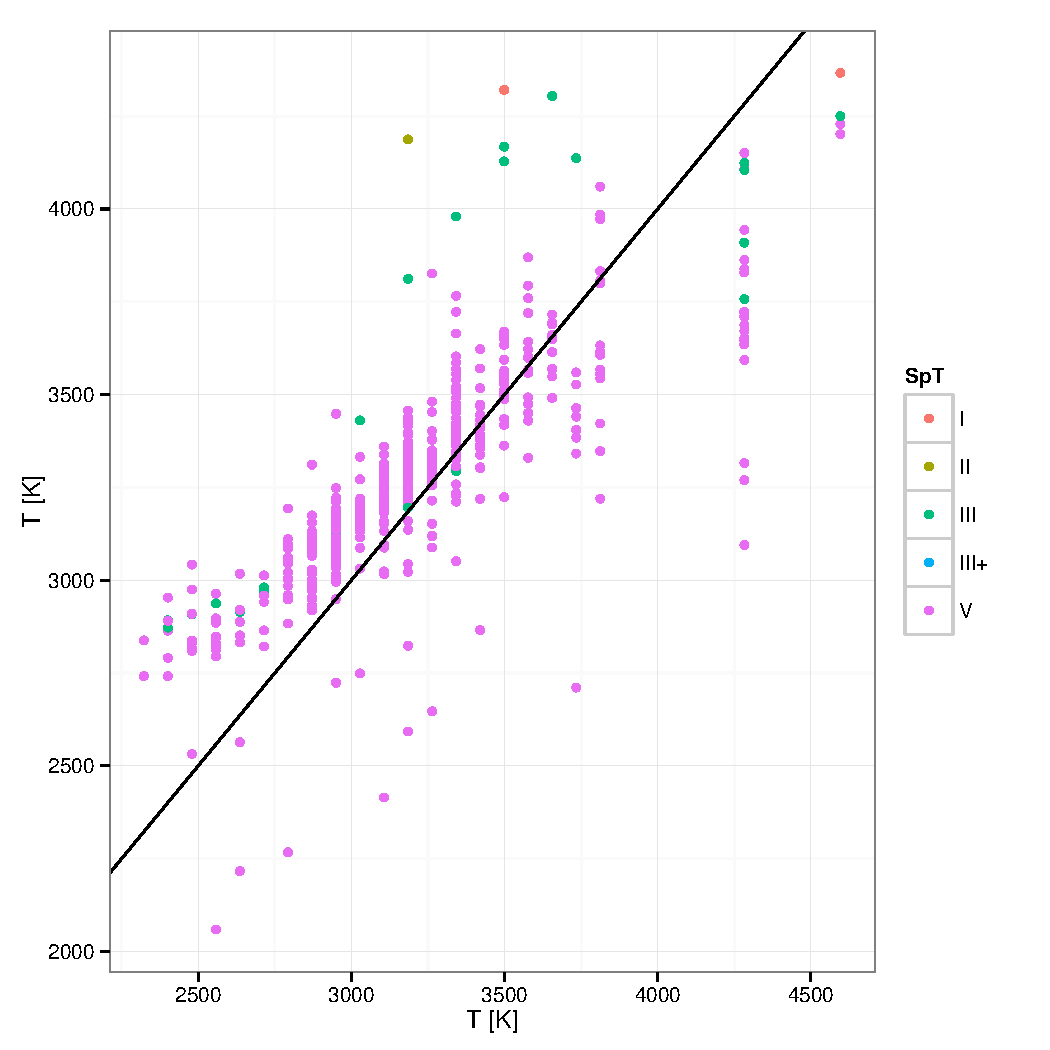
\includegraphics[width=6cm]{figs/T10GA_TSB.pdf}
%  \caption{Comparison between Temperature estimations from Spectral Subtype 
%  in x axis and the Random Forest for Ga based features trained with BT-Settl 
%  at SNR=10 on y-axis}
%  \label{fig:t10ga_tsb}
%  \end{center}
% \end {figure}


The comparison against processing the whole spectrum by ICA projection 
has been performed and the results for SNR=\{10,50\} can be seen 
in Figure~\ref{fig:T_ICA_10_SpT} and Figure~\ref{fig:T_ICA_50_SpT}.

\begin {figure}
 \centering
 \begin{subfigure}{.85\textwidth}
  \centering
  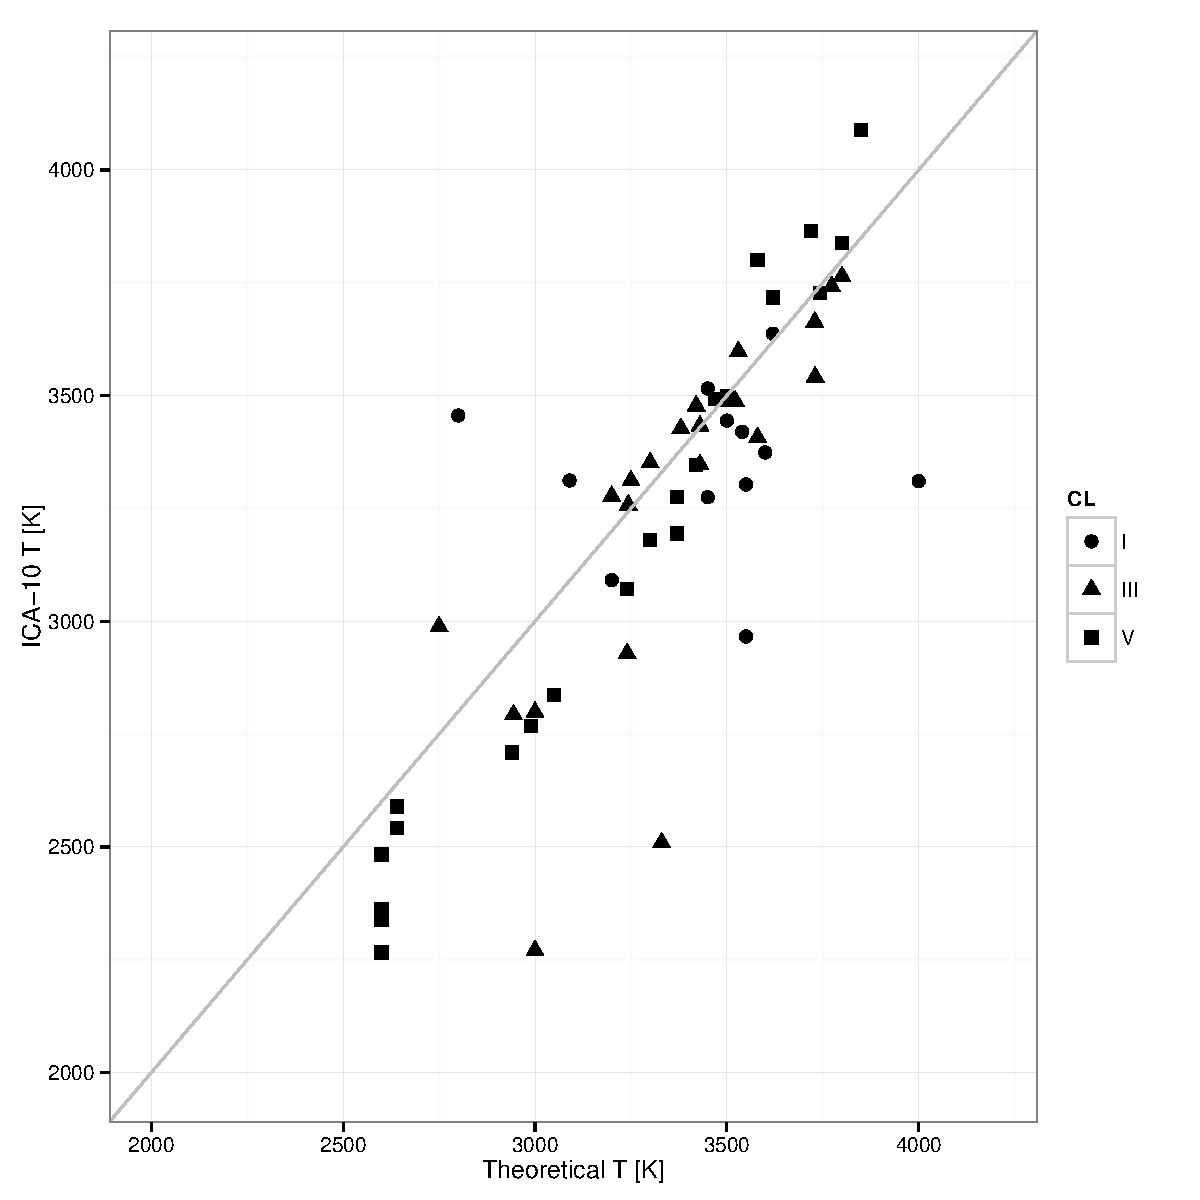
\includegraphics[width=12cm]{figs/T_ICA_10_SpT.pdf}
  \caption{Comparison between Temperature estimations from Spectral Subtype 
 in x axis and the prediction based on SVM models over the ICA projection 
 with 10 components at SNR=$10$ on y-axis}
 \label{fig:T_ICA_10_SpT}
 \end{subfigure}
  \begin{subfigure}{.85\textwidth}
   \centering
  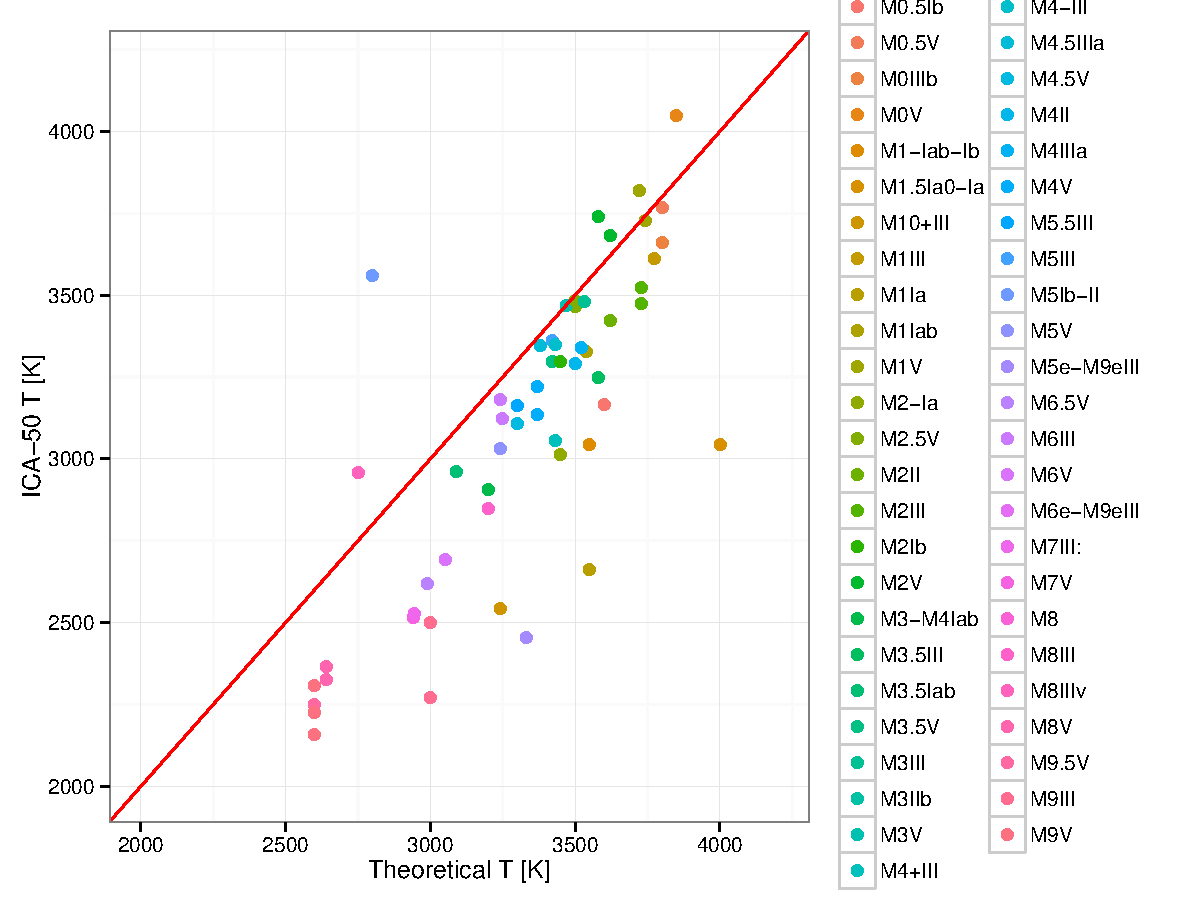
\includegraphics[width=12cm]{figs/T_ICA_50_SpT.pdf}
  \caption{Comparison between Temperature estimations from Spectral Subtype 
 in x axis and the prediction based on SVM models over the ICA projection 
 with 10 components at SNR=$50$ on y-axis}
 \label{fig:T_ICA_10_SpT}  
  \end{subfigure}
 \label{fig:t_ica_1050_SpT}
\end {figure}

% No le añado más discusión de momento, hasta ver si tiene sentido poer toda esta
% fila de gráficas o es mejor producir algo más condensado.
%
}



{
The same approach can become useful to produce $log(G)$ estimations. 
Here comparisons can only be possible between GA based features, the 
global spectra based approach with $\chi^2$ distance
to be minimized and those stars with gravity was 
estimated in  \cite{2013A&A...549A.129C}.

The only difference with the methodology presented above is because
Temperature has been considered a fixed feature in the estimation of 
Gravity.

In Tables~\ref{tab:models_G_rmse} and~\ref{tab:models_G_mae} 
we can see the analysis of performance between
the $\chi^2$ identificacion and the one based on features from the spectrum
depending on several classes of features.

\begin{table}[ht]
\centering
\begin{tabular}{rrrrrrrr}
  \hline
 & rf & gbm & boosting & svm & gam & nnet & mars \\ 
  \hline
G\_chi2\_10 & 1.68 & 1.68 & 1.68 & 1.68 & 1.68 & 1.68 & 1.68 \\ 
  G\_chi2\_50 & 1.79 & 1.79 & 1.79 & 1.79 & 1.79 & 1.79 & 1.79 \\ 
  FG00 & 2.01 & 1.62 & 2.32 & 1.78 & 0.98 & 3.39 & 2.13 \\ 
  FG01 & 2.52 & 2.56 & 2.62 & 1.87 & 2.52 & 2.32 & 2.45 \\ 
  FG05 & 2.49 & 2.42 & 2.40 & 1.78 & 2.29 & 2.89 & 2.16 \\ 
  FG10 & 2.34 & 2.59 & 2.75 & 1.78 & 32.52 & 3.39 & 3.04 \\ 
  FG11 & 2.49 & 2.48 & 2.69 & 1.90 & 2.67 & 2.50 & 2.57 \\ 
  FG15 & 2.75 & 2.72 & 2.51 & 1.78 & 2.95 & 3.94 & 2.52 \\ 
  FG50 & 2.61 & 2.11 & 2.58 & 1.78 & 17.95 & 3.39 & 6.07 \\ 
  FG51 & 2.78 & 2.82 & 2.77 & 1.92 & 2.73 & 2.43 & 2.65 \\ 
  FG55 & 2.58 & 2.57 & 2.71 & 1.78 & 2.80 & 2.34 & 2.63 \\ 
   \hline
\end{tabular}
\caption { RMSE for different models predicting $Log(G)$ [dex].} 
\label{tab:models_G_rmse} 
\end{table}

\begin{table}[ht]
\centering
\begin{tabular}{rrrrrrrr}
  \hline
 & rf & gbm & boosting & svm & gam & nnet & mars \\ 
  \hline
G\_chi2\_10 & 1.46 & 1.46 & 1.46 & 1.46 & 1.46 & 1.46 & 1.46 \\ 
  G\_chi2\_50 & 1.46 & 1.46 & 1.46 & 1.46 & 1.46 & 1.46 & 1.46 \\ 
  FG00 & 1.78 & 1.50 & 2.05 & 1.54 & 0.82 & 3.06 & 1.84 \\ 
  FG01 & 2.14 & 2.19 & 2.27 & 1.75 & 2.18 & 1.80 & 2.07 \\ 
  FG05 & 2.13 & 2.07 & 2.07 & 1.35 & 1.59 & 2.70 & 1.54 \\ 
  FG10 & 2.09 & 2.31 & 2.43 & 1.54 & 27.48 & 3.06 & 2.73 \\ 
  FG11 & 2.12 & 2.16 & 2.34 & 1.77 & 2.30 & 2.03 & 2.17 \\ 
  FG15 & 2.35 & 2.29 & 2.17 & 1.35 & 2.52 & 3.64 & 1.86 \\ 
  FG50 & 2.50 & 1.99 & 2.23 & 1.54 & 15.75 & 3.06 & 4.03 \\ 
  FG51 & 2.46 & 2.48 & 2.43 & 1.79 & 2.50 & 1.89 & 2.37 \\ 
  FG55 & 2.15 & 2.16 & 2.34 & 1.35 & 2.48 & 2.05 & 2.29 \\ 
   \hline
\end{tabular}
\caption { RMSE for different models predicting $Log(G)$ [dex].} 
\label{tab:models_G_mae} 
\end{table}


In Figure~\ref{fig:chi2_50_spt} and Figure~\ref{fig:ga_too50ga_spt} 
relationships between $log(g)$ predicted by global espectrum estimation 
and GA feature based estimation can be observed.

\begin {figure}
 \centering
 \begin{subfigure}{.85\textwidth}
  \centering
  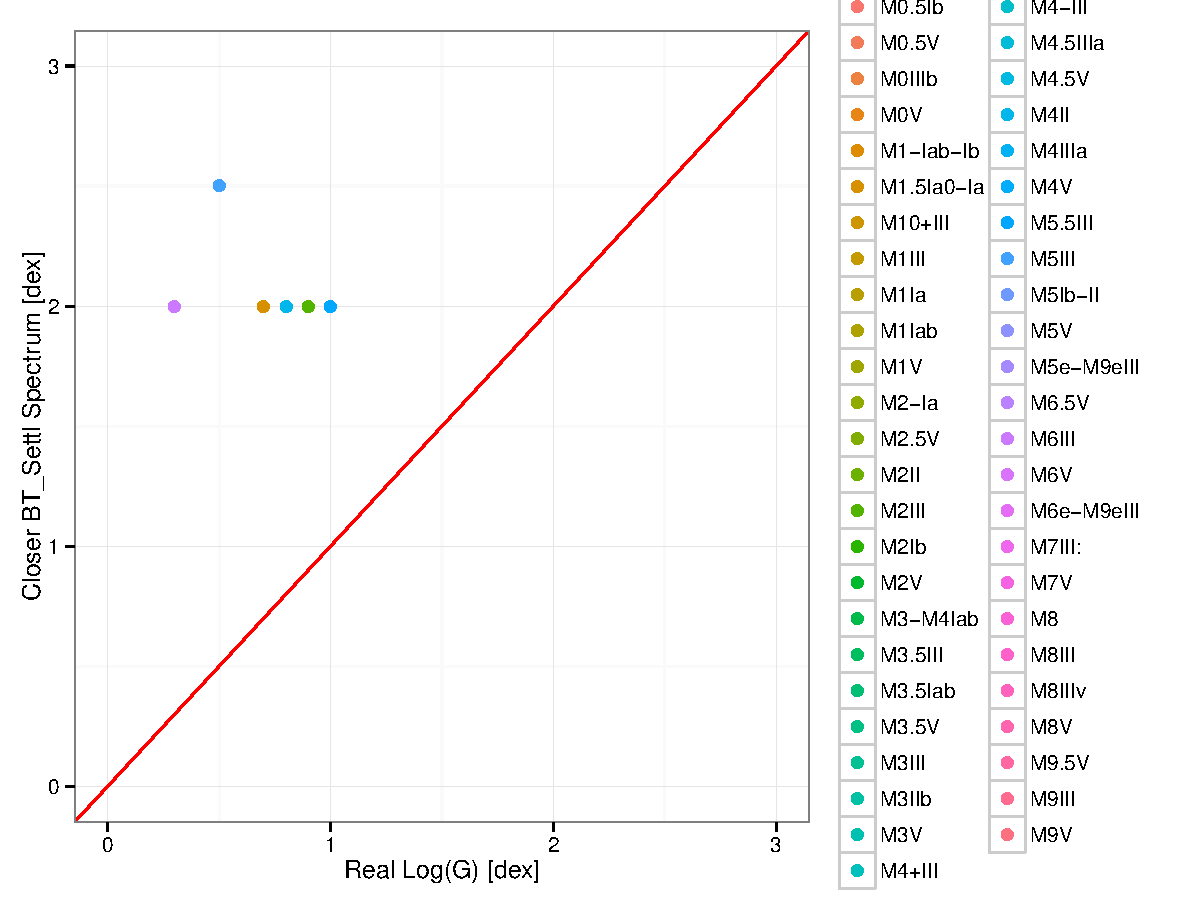
\includegraphics[width=12cm]{figs/G_chi2_50_cesetti.pdf}
  \caption{Comparison between Gravity estimations from Spectral Subtype 
 in x axis and the closest BT\_Settl spectra by $\chi^2$ at SNR=$50$ on y-axis}
 \label{fig:chi2_50_spt}
 \end{subfigure}
  \begin{subfigure}{.85\textwidth}
  \centering
  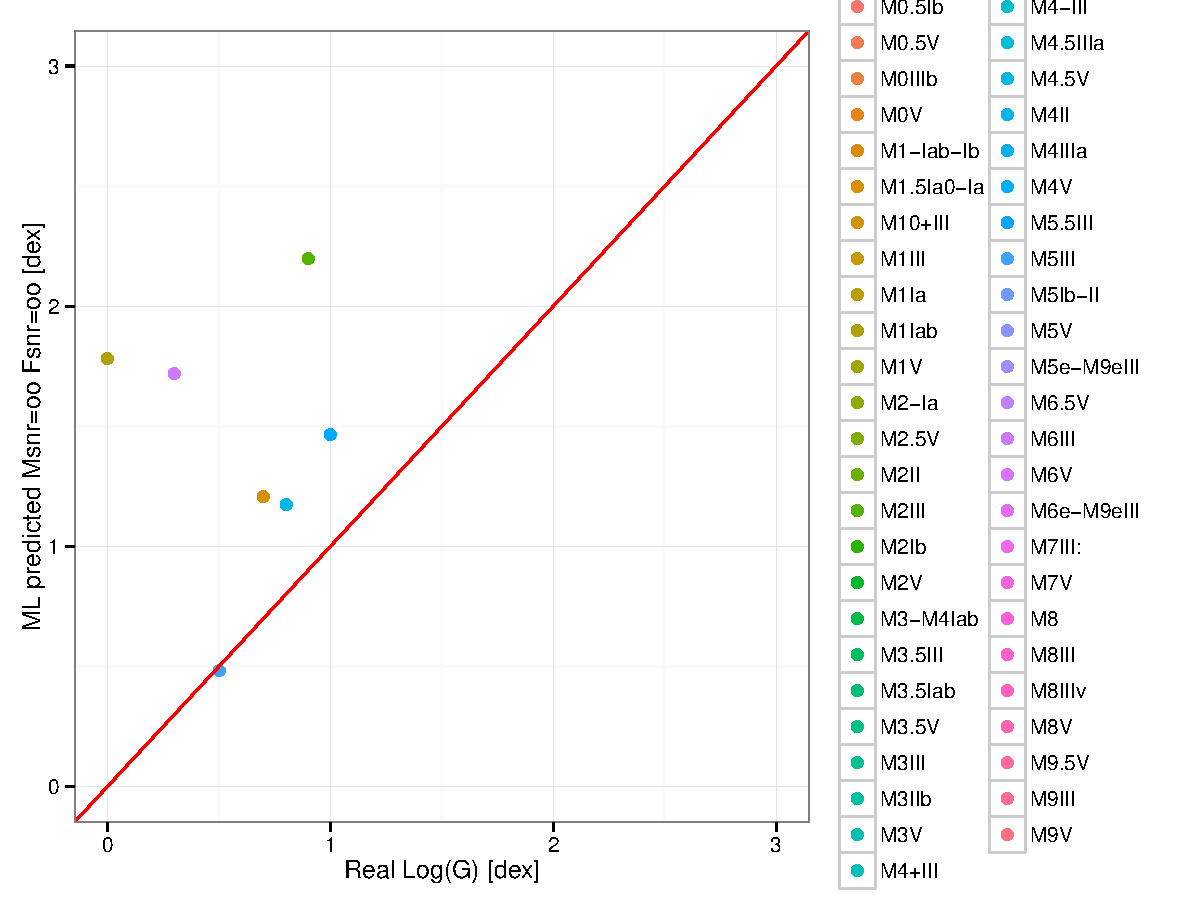
\includegraphics[width=12cm]{figs/G_gam_oo_cesetti.pdf}
  \caption{Comparison between Gravity estimations from Spectral Subtype 
 in x axis and the Support Vector Machines for Ga based features trained with BT\_Settl 
 at SNR=$\infty$ and features for forecasting at SNR=$\infty$ on y-axis}
 \label{fig:ga_too50ga_spt}
 \end{subfigure}
 \label {fig:comp02}
 \caption{Performance comparison between the $chi^2$ based selection 
          and the band oriented features to forecast Log(g)}
\end {figure}
%

% De nuevo las valoraciones deberían esperar a ver qué ponemos.

}

{ 

Finally, the same analysis is performed for the Metalicty parameter, 
again by considering Temperature as a fixed feature.
In Tables~\ref{tab:models_M_rmse} and~\ref{tab:models_M_mae} 
we can see the analysis of performance of different classes of
models and cosidering a variety in features.

\begin{table}[ht]
\centering
\begin{tabular}{rrrrrrrr}
  \hline
 & rf & gbm & boosting & svm & gam & nnet & mars \\ 
  \hline
M\_Chi2\_10 & 0.19 & 0.19 & 0.19 & 0.19 & 0.19 & 0.19 & 0.19 \\ 
 M\_Chi2\_50 & 0.35 & 0.35 & 0.35 & 0.35 & 0.35 & 0.35 & 0.35 \\ 
  FM00 & 0.30 & 0.43 & 0.28 & 1.04 & 2.19 & 0.51 & 1.03 \\ 
  FM01 & 0.51 & 0.46 & 0.44 & 0.74 & 0.76 & 0.99 & 50.64 \\ 
  FM05 & 2.05 & 2.85 & 1.31 & 1.89 & 3.46 & 7.56 & 6.46 \\ 
  FM10 & 1.09 & 1.02 & 0.94 & 1.04 & 10.75 & 1.65 & 13.49 \\ 
  FM11 & 0.47 & 0.39 & 0.49 & 0.74 & 0.31 & 0.45 & 43.43 \\ 
  FM15 & 1.91 & 2.73 & 1.08 & 1.89 & 4.65 & 13.27 & 16.95 \\ 
  FM50 & 0.82 & 0.87 & 0.43 & 1.04 & 6.10 & 2.25 & 11.87 \\ 
  FM51 & 1.02 & 1.10 & 0.56 & 0.74 & 2.29 & 3.44 & 119.29 \\ 
  FM55 & 1.70 & 3.14 & 1.15 & 1.89 & 7.64 & 7.00 & 12.04 \\ 
   \hline
   \end{tabular}
\caption { RMSE for different models predicting $Met$ [dex].} 
\label{tab:models_M_rmse} 
\end{table}
   


\begin{table}[ht]
\centering
\begin{tabular}{rrrrrrrr}
  \hline
 & rf & gbm & boosting & svm & gam & nnet & mars \\ 
  \hline
M\_Chi2\_10 & 0.17 & 0.17 & 0.17 & 0.17 & 0.17 & 0.17 & 0.17 \\ 
  M\_Chi2\_50 & 0.26 & 0.26 & 0.26 & 0.26 & 0.26 & 0.26 & 0.26 \\ 
  FM00 & 0.24 & 0.38 & 0.25 & 1.02 & 2.01 & 0.33 & 0.92 \\ 
  FM01 & 0.47 & 0.40 & 0.40 & 0.72 & 0.66 & 0.90 & 33.30 \\ 
  FM05 & 2.04 & 2.85 & 1.29 & 1.88 & 3.41 & 7.38 & 6.28 \\ 
  FM10 & 0.80 & 0.71 & 0.62 & 1.02 & 8.88 & 0.99 & 10.82 \\ 
  FM11 & 0.43 & 0.37 & 0.46 & 0.72 & 0.24 & 0.37 & 25.59 \\ 
  FM15 & 1.90 & 2.68 & 1.05 & 1.88 & 3.68 & 11.77 & 13.21 \\ 
  FM50 & 0.78 & 0.79 & 0.40 & 1.02 & 5.13 & 1.83 & 9.90 \\ 
  FM51 & 1.01 & 1.08 & 0.54 & 0.72 & 2.22 & 3.36 & 77.52 \\ 
  FM55 & 1.67 & 3.10 & 1.13 & 1.88 & 7.11 & 6.33 & 11.22 \\
   \hline
   \end{tabular}
\caption { MAE for different models predicting $Met$ [dex].} 
\label{tab:models_M_mae} 
\end{table}
   

In Figure~\ref{fig:M_chi2_50_cesetti} and Figure~\ref{fig:M_GAM_1010_Cesetti} 
relationships between metalicity predicted by global espectrum estimation 
and GA feature based estimation against the real values
provided by \cite{2013A&A...549A.129C} can be observed.

\begin {figure}
 \centering
 \begin{subfigure}{.85\textwidth}
  \centering
  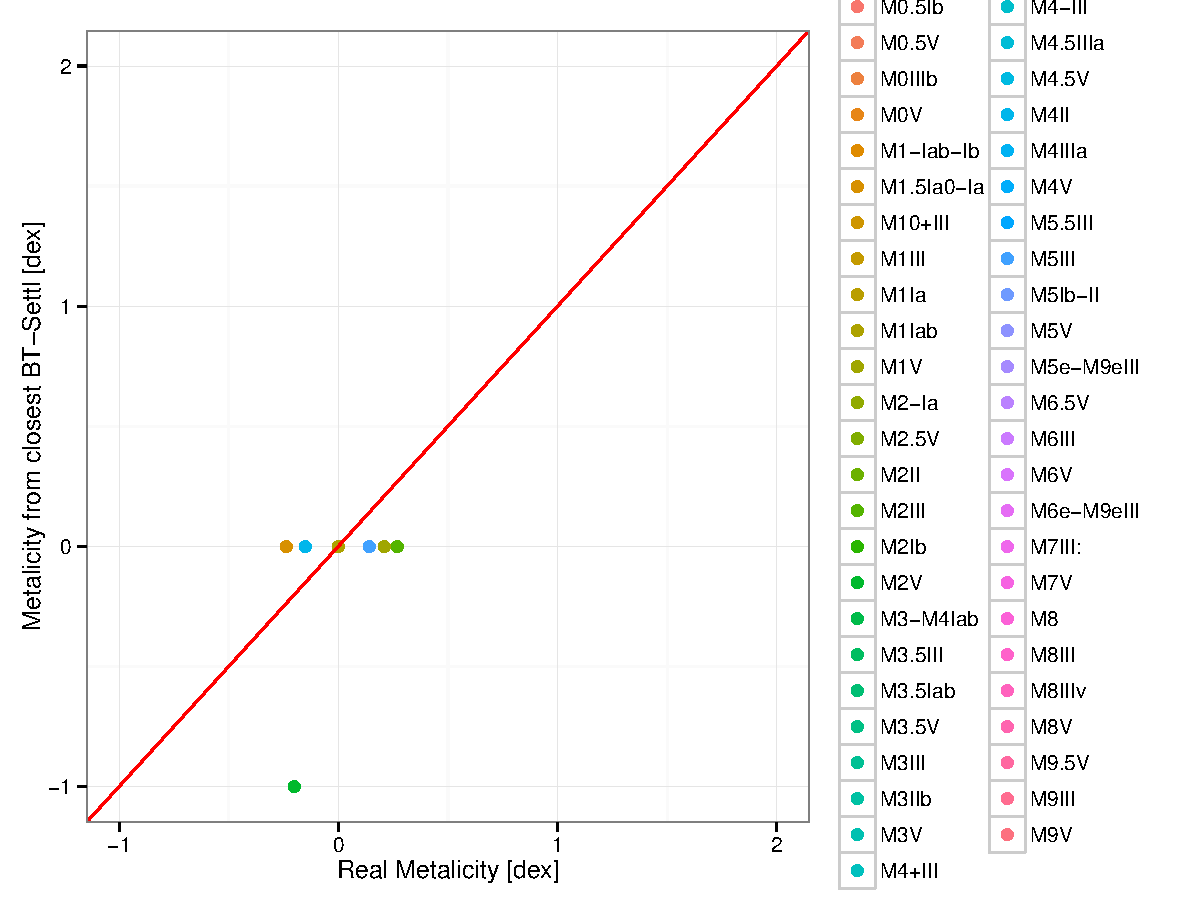
\includegraphics[width=12cm]{figs/M_Chi2_50_Cesetti.pdf}
  \caption{Comparison between Metalicity estimations from Spectral Subtype 
 in x axis and the closest BT\_Settl spectra by $\chi^2$ at SNR=$50$ on y-axis}
 \label{M_chi2_50_cesetti}
 \end{subfigure}
  \begin{subfigure}{.85\textwidth}
  \centering
  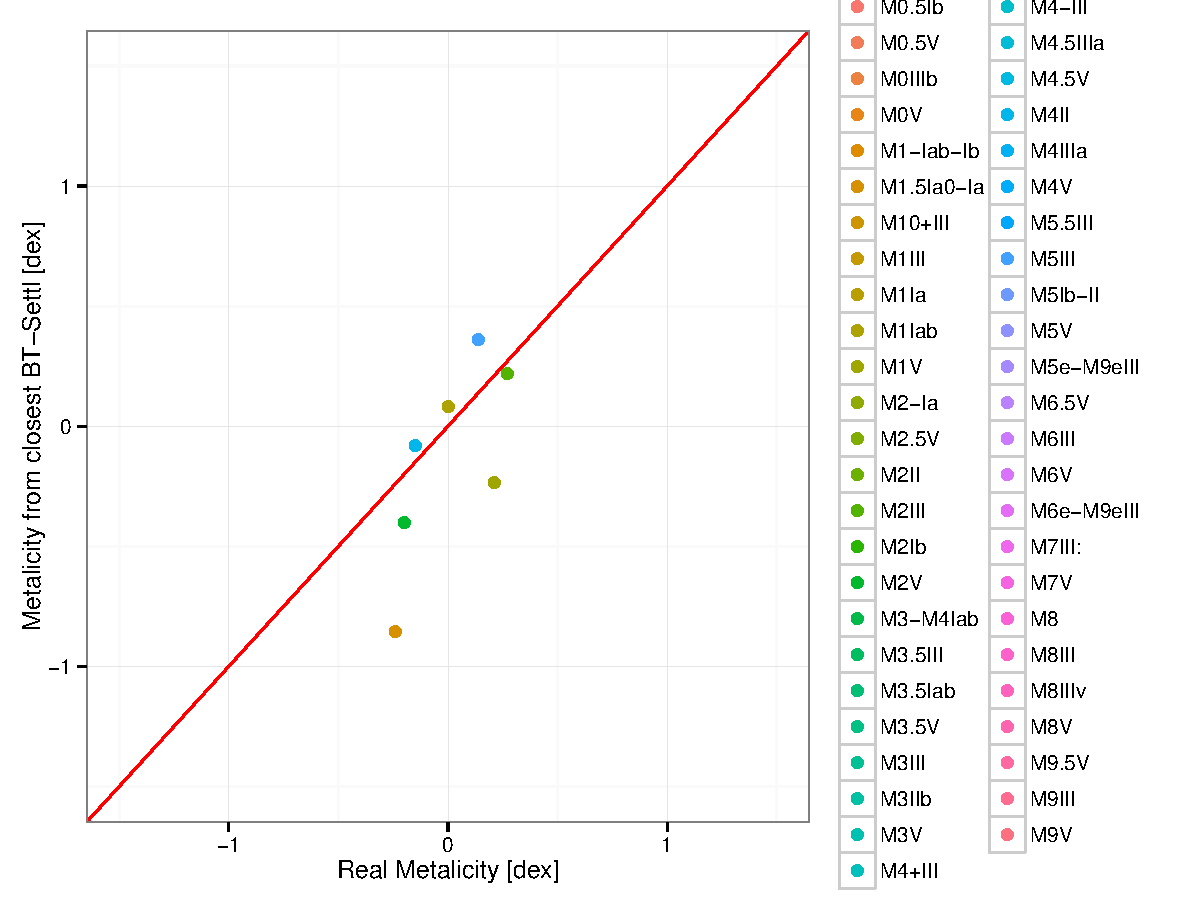
\includegraphics[width=12cm]{figs/M_GAM_1010_Cesetti.pdf}
  \caption{Comparison between Metalicity estimations from Spectral Subtype 
 in x axis and the Support Vector Machines for Ga based features trained with BT\_Settl 
 at SNR=$\infty$ and features for forecasting at SNR=$\infty$ on y-axis}
 \label{fig:M_GAM_1010_Cesetti}
 \end{subfigure}
 \label {fig:comp03}
 \caption{Performance comparison between the $chi^2$ based selection 
          and the band oriented features to forecast Log(g)}
\end {figure}
%
   
   

% De nuevo, el análisis y discusión, función de lo que queramos dejar
}

{
It is possible to present relationships between $log(g)$ and $log(T_{eff})$
as a matter of congruence analysis between predictions. In the Figure~\ref{fig:lt_lg_ga}
such relationship is presented for models based on artificial intelligence selected features.
In Figure~\ref{fig:lt_lg_chi2} the values for $log(T_{eff})$ and $log(G)$ are 
inferred from the closest BT\_Settl spectra.

\begin{figure}
 \begin{center}
 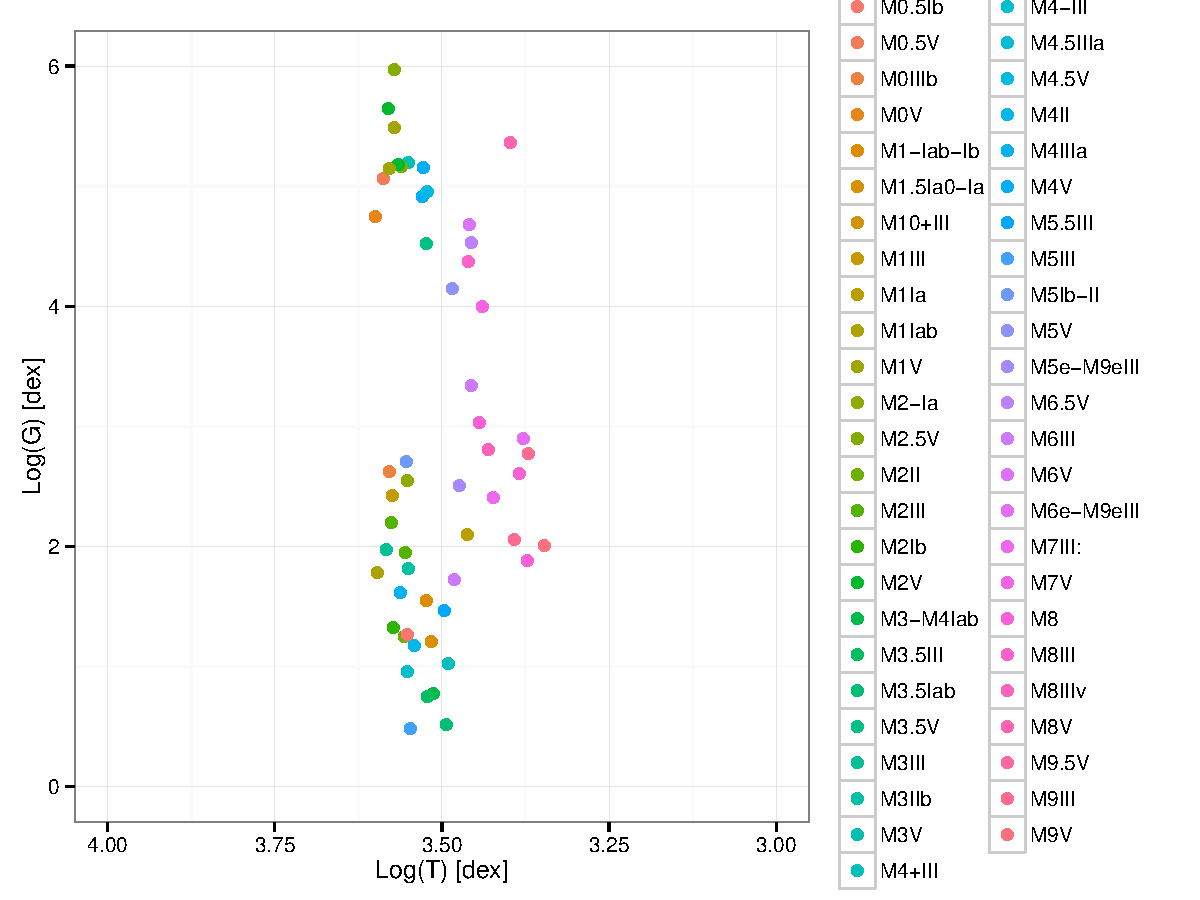
\includegraphics[width=12cm]{figs/LT_LG_ga.pdf}
 \caption{Relationship between $log(T_{eff}) $ in the x axis 
 and $log(g)$ in the y axis for models based on bandpass features }
 \label{fig:lt_lg_ga}
 \end{center}
\end{figure}

And, for sure, it is possible to do it for estimations based on 
parameters from nearest labeled BT-Settl spectra.
In this particular case, it is possible to see how 
considering the global spectrum is positive for stronger 
physical parameters like $T_{eff}$ but the approach
reduces drastically its likelihood when other softer 
parameters are involved.

\begin{figure}
 \begin{center}
 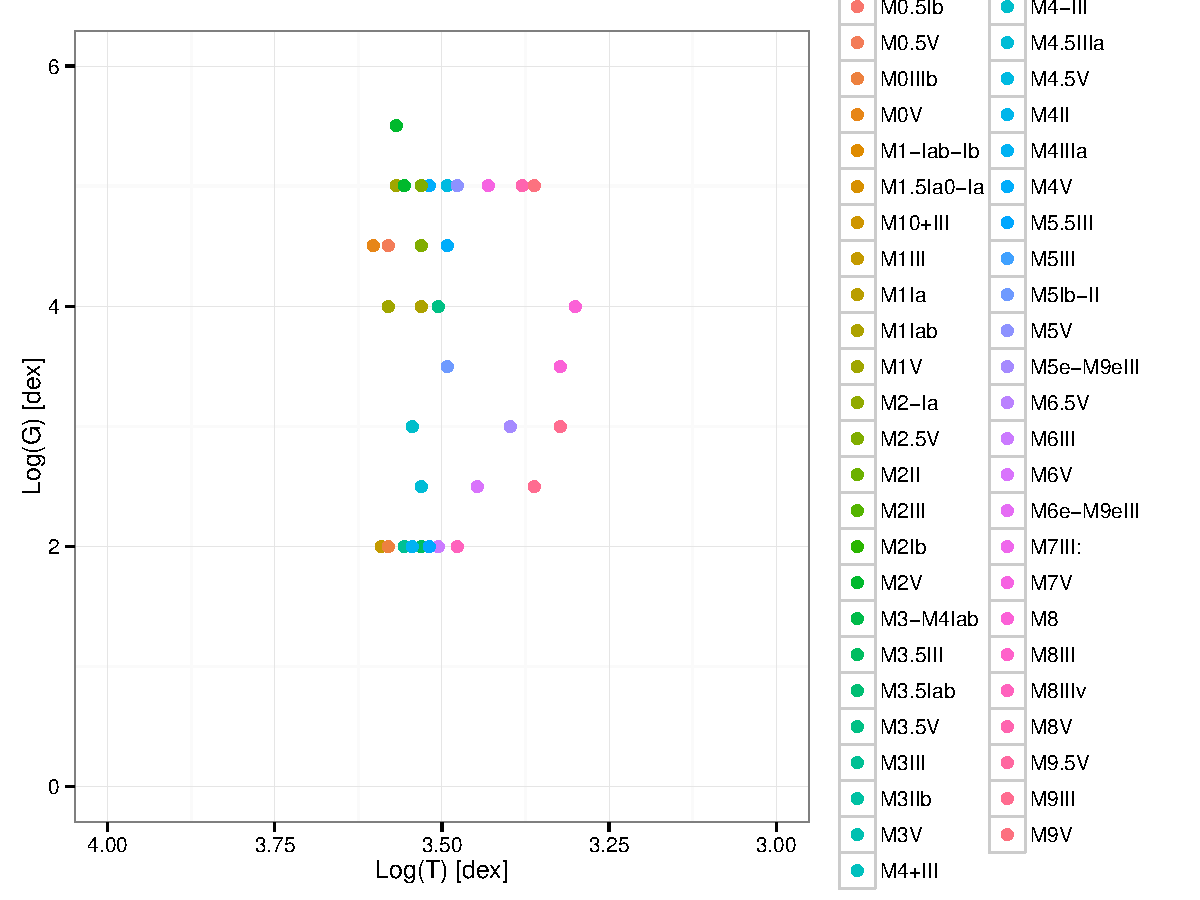
\includegraphics[width=12cm]{figs/LT_LG_chi2.pdf}
 \caption{Relationship between $log(T_{eff}) $ in the x axis 
 and $log(g)$ in the y axis for SNR=50 when 
 the nearest BT-Settl spectrum is used.}
 \label{fig:lt_lg_chi2}
 \end{center}
\end{figure}

% Se debe realizar una intepretación, pero dependerá 

}